\chapter{\selectlanguage{greek}Θεωρητικό Υπόβαθρο}
Κατηγοριοποίηση Εικόνων με χρήση Συνελικτικών Νευρωνικών Δικτύων  
\en{classifying images using a Convolutional Neural Network}

\section{Αναγνώριση Εικόνων}
\subsection{Πώς ένας υπολογιστής αναγνωρίζει εικόνες;}
Η ταξινόμηση εικόνων περιγράφει ένα πρόβλημα στο οποίο σε ένα υπολογιστή δίνεται μία εικόνα και πρέπει να καταλάβει τι απεικονίζει (από ένα σύνολο πιθανών κατηγοριών)
Σήμερα, τα Συνελικτικά Νευρωνικά Δίκτυα (\en{CNNs}) αποτελούν  μια πολύ καλή  προσέγγιση αυτού το προβλήματος. Γενικά, τα νευρωνικά δίκτυα υποθέτουν πως υπάρχει κάποια συνάρτηση από την είσοδο (π.χ. εικόνες) σε μία έξοδο (π.χ. ένα σύνολο κατηγοριών εικόνων). Ενώ οι κλασσικοί αλγόριθμοι προσπαθούν να κωδικοποιήσουν  κάποια πληροφορία του πραγματικού κόσμου στη συνάρτηση τους, τα \en{CNN} μαθαίνουν την συνάρτηση δυναμικά  από ένα σύνολο ταξινομημένων εικόνων (\en{labelled images})—αυτή η διαδικασία ονομάζετε εκπαίδευση. Μόλις καταλήξει σε μια σταθερή συνάρτηση (δηλαδή σε μια προσέγγιση αυτής), μπορεί να εφαρμόσει τη συνάρτηση σε εικόνες που δεν έχει ξαναδεί.
\subsection{Τι μπορεί να κάνει ένα νευρωνικό δίκτυο;}
Ένα νευρωνικό δίκτυο αποτελείται από πολλαπλά επίπεδα.  Κάθε επίπεδο λαμβάνει έναν πολυδιάστατο πίνακα αριθμών ως είσοδο και παράγει έναν άλλο πολυδιάστατο πίνακα αριθμών ως έξοδο (ο οποίος στη συνέχεια γίνεται η είσοδος του επόμενου επιπέδου). Κατά την ταξινόμηση εικόνων, η είσοδος του πρώτου επιπέδου είναι η εικόνα εισόδου  (π.χ. 32\en{x}32\en{x}3 αριθμοί για εικόνες 32\en{x}32 \en{pixel} με 3 κανάλια χρώματος), ενώ η έξοδος του τελευταίου επιπέδου αποτελείται  ένα σύνολο πιθανοτήτων των διαφόρων κατηγοριών (π.χ., 1\en{x}1\en{x}10 αριθμοί αν υπάρχουν 10 κατηγορίες).

\begin{figure}[!ht] \centering 
%\includegraphics[width=\textwidth]{universe}
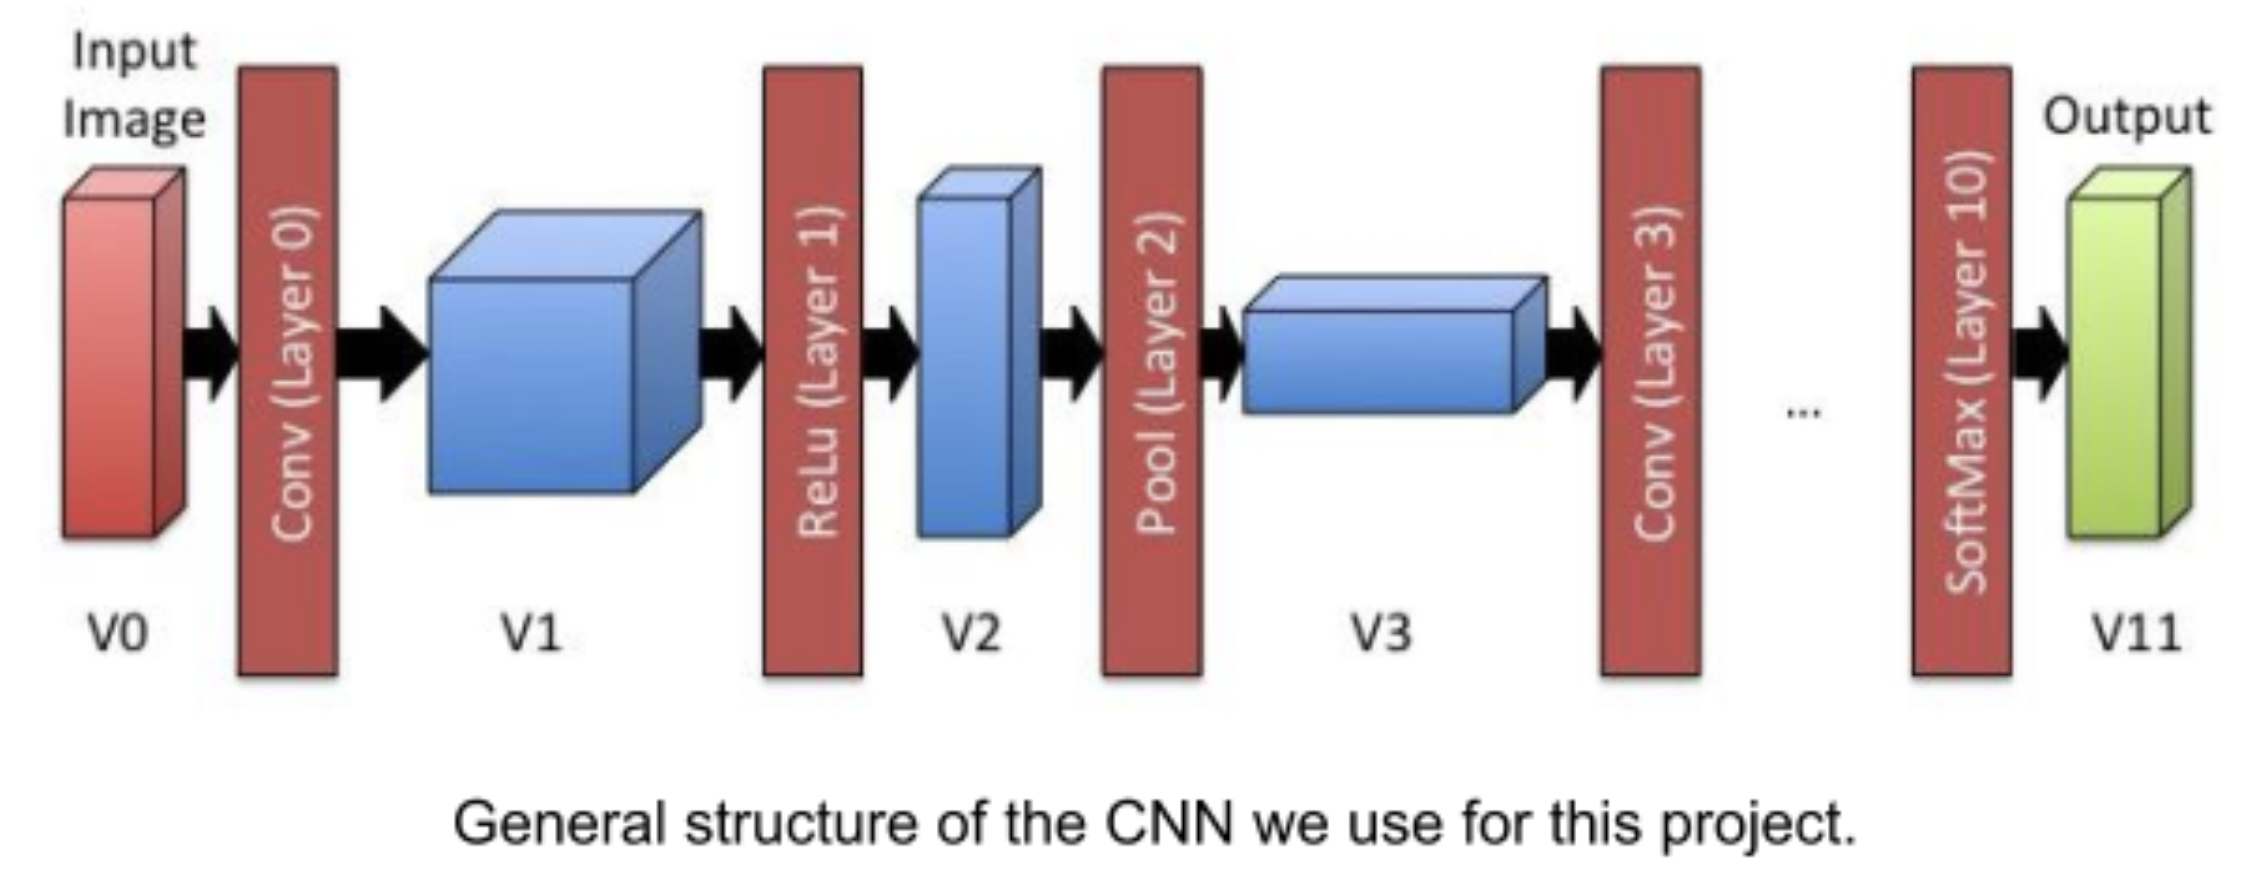
\includegraphics[width=\textwidth]{static/figures/network.png} \caption{Δομή Συνελικτικού Νευρωνικού Δικτύου}\label{figureCNN}
\end{figure}

Αρχιτεκτονική \en{CNN}~\ref{figureCNN} 

Κάθε επίπεδο έχει ένα σύνολο από βάρη που σχετίζονται με αυτό — αυτά τα βάρη είναι που “μαθαίνει” το νευρωνικό όταν του δοθούν δεδομένα εκπαίδευσης. Ανάλογα με το επίπεδο, τα βάρη έχουν διαφορετικές ερμηνείες, αλλά δεν είναι αντικείμενο μελέτης του συγκεκριμένου \en{project}, φτάνει να γνωρίζουμε ότι κάθε επίπεδο λαμβάνει μία είσοδο, εκτελεί κάποια διεργασία σε αυτή, που εξαρτάται από τα βάρη και παράγει μια έξοδο. Αυτό το βήμα ονομάζεται \en{forward pass}: παίρνουμε μία είσοδο και την προωθούμε στο δίκτυο, παράγοντας το επιθυμητό αποτέλεσμα ως έξοδο. Το \en{forward pass} είναι το μόνο που χρειάζεται για την ταξινόμηση εικόνων σε ένα ήδη εκπαιδευμένο \en{CNN}.
    

Στην πράξη, ένα νευρωνικό δίκτυο αποτελεί μια πολύ απλή μηχανή αναγνώρισης προτύπων (με εξαιρετικά περιορισμένη χωρητικότητα), αλλά μπορεί να είναι αρκετά παράξενο αυτό που καταλήγει να αναγνωρίσει. Για παράδειγμα, κάποιος μπορεί να εκπαιδεύσει ένα νευρωνικό δίκτυο να αναγνωρίζει τη διαφορά μεταξύ “σκύλων” και “λύκων”, και να δουλέψει καλά κοιτώντας το χιόνι και το δάσος στο φόντο των φωτογραφιών με τους λύκους.

